\section{Reliability diagrams}
\lb{sec:reliability}


\begin{figure*}[ht]
\centering
\hspace*{-0.5cm}
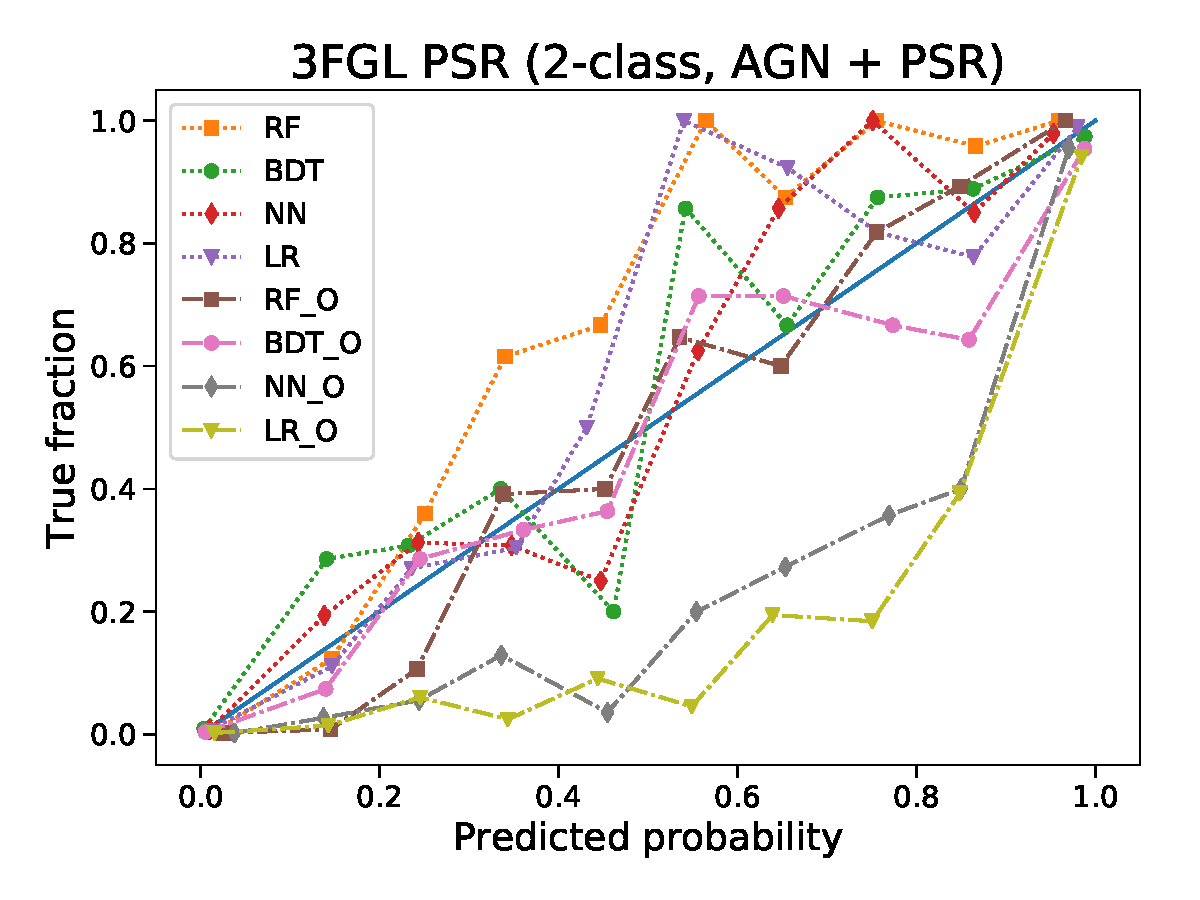
\includegraphics[width=0.45\textwidth]{plots/reliability/calibration_PSR_3FGL_2classes_AGN_PSR.pdf}
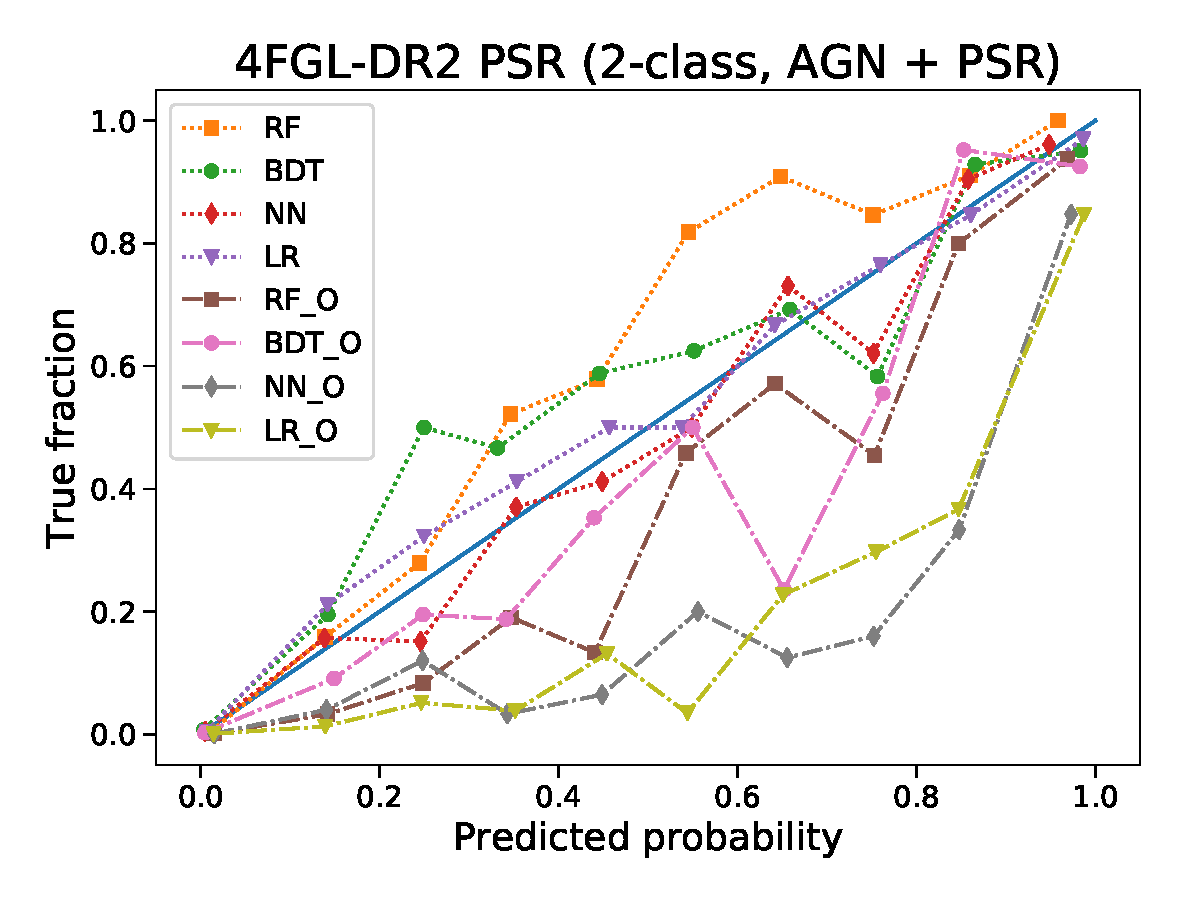
\includegraphics[width=0.45\textwidth]{plots/reliability/calibration_PSR_4FGL-DR2_2classes_AGN_PSR.pdf} \\ 
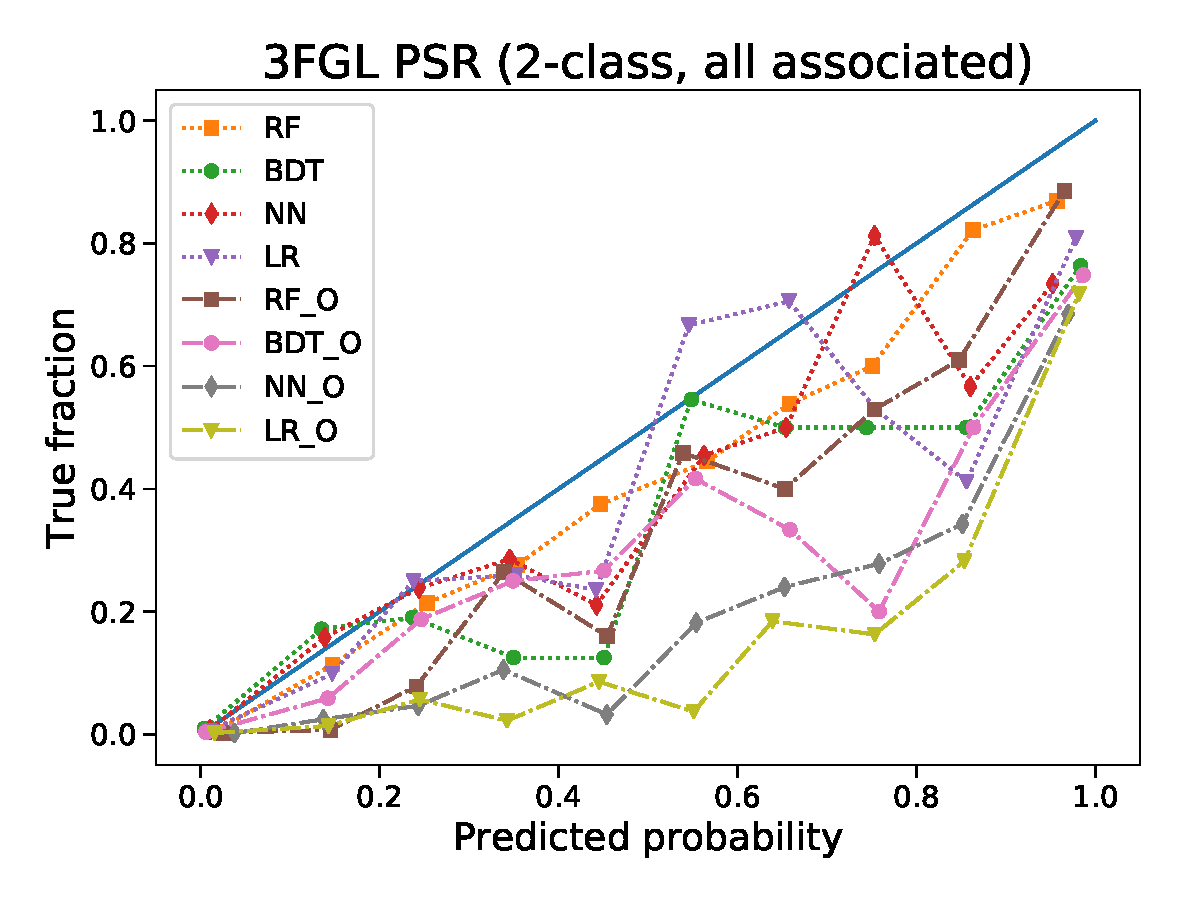
\includegraphics[width=0.45\textwidth]{plots/reliability/calibration_PSR_3FGL_2classes_all_assoc.pdf}
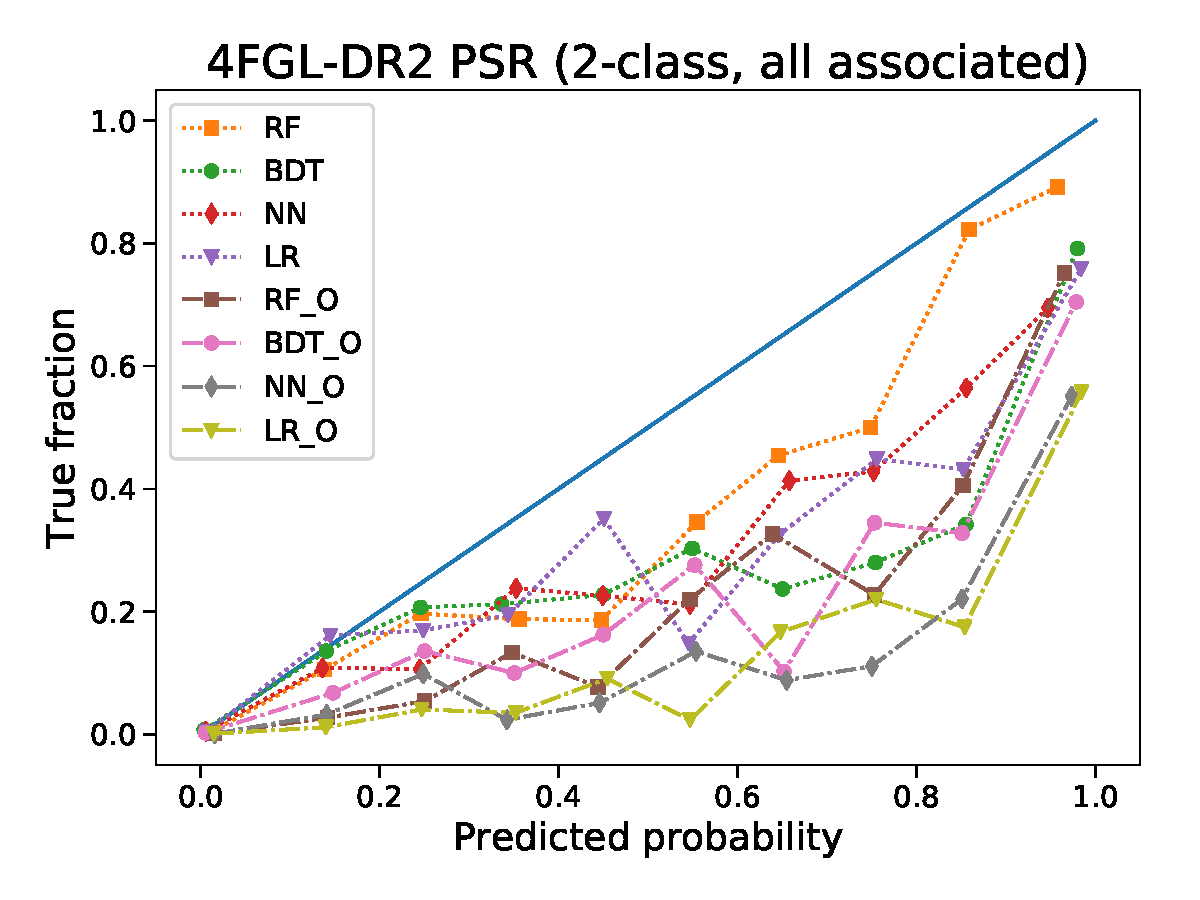
\includegraphics[width=0.45\textwidth]{plots/reliability/calibration_PSR_4FGL-DR2_2classes_all_assoc.pdf} \\ 
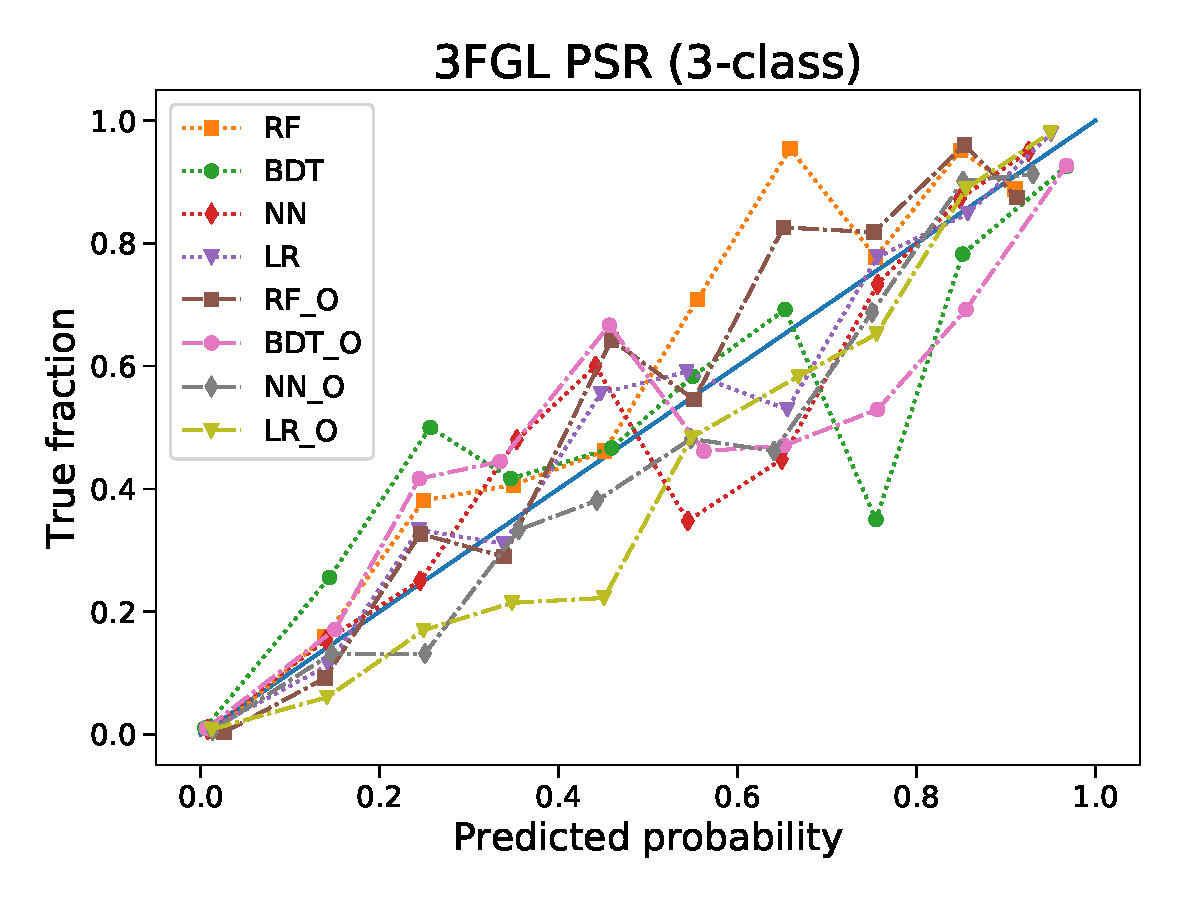
\includegraphics[width=0.45\textwidth]{plots/reliability/calibration_PSR_3FGL_3classes.pdf}
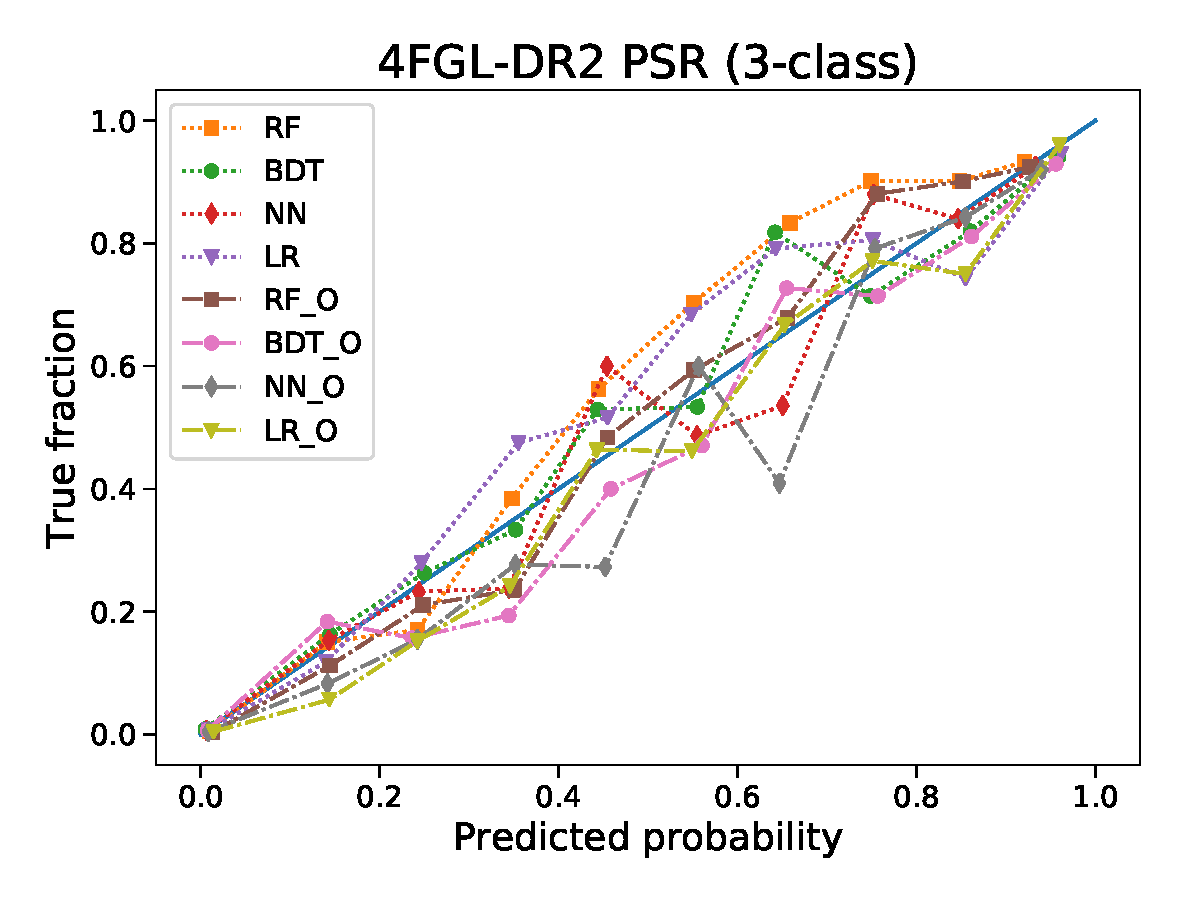
\includegraphics[width=0.45\textwidth]{plots/reliability/calibration_PSR_4FGL-DR2_3classes.pdf}
	%\hspace*{-0.5cm}
%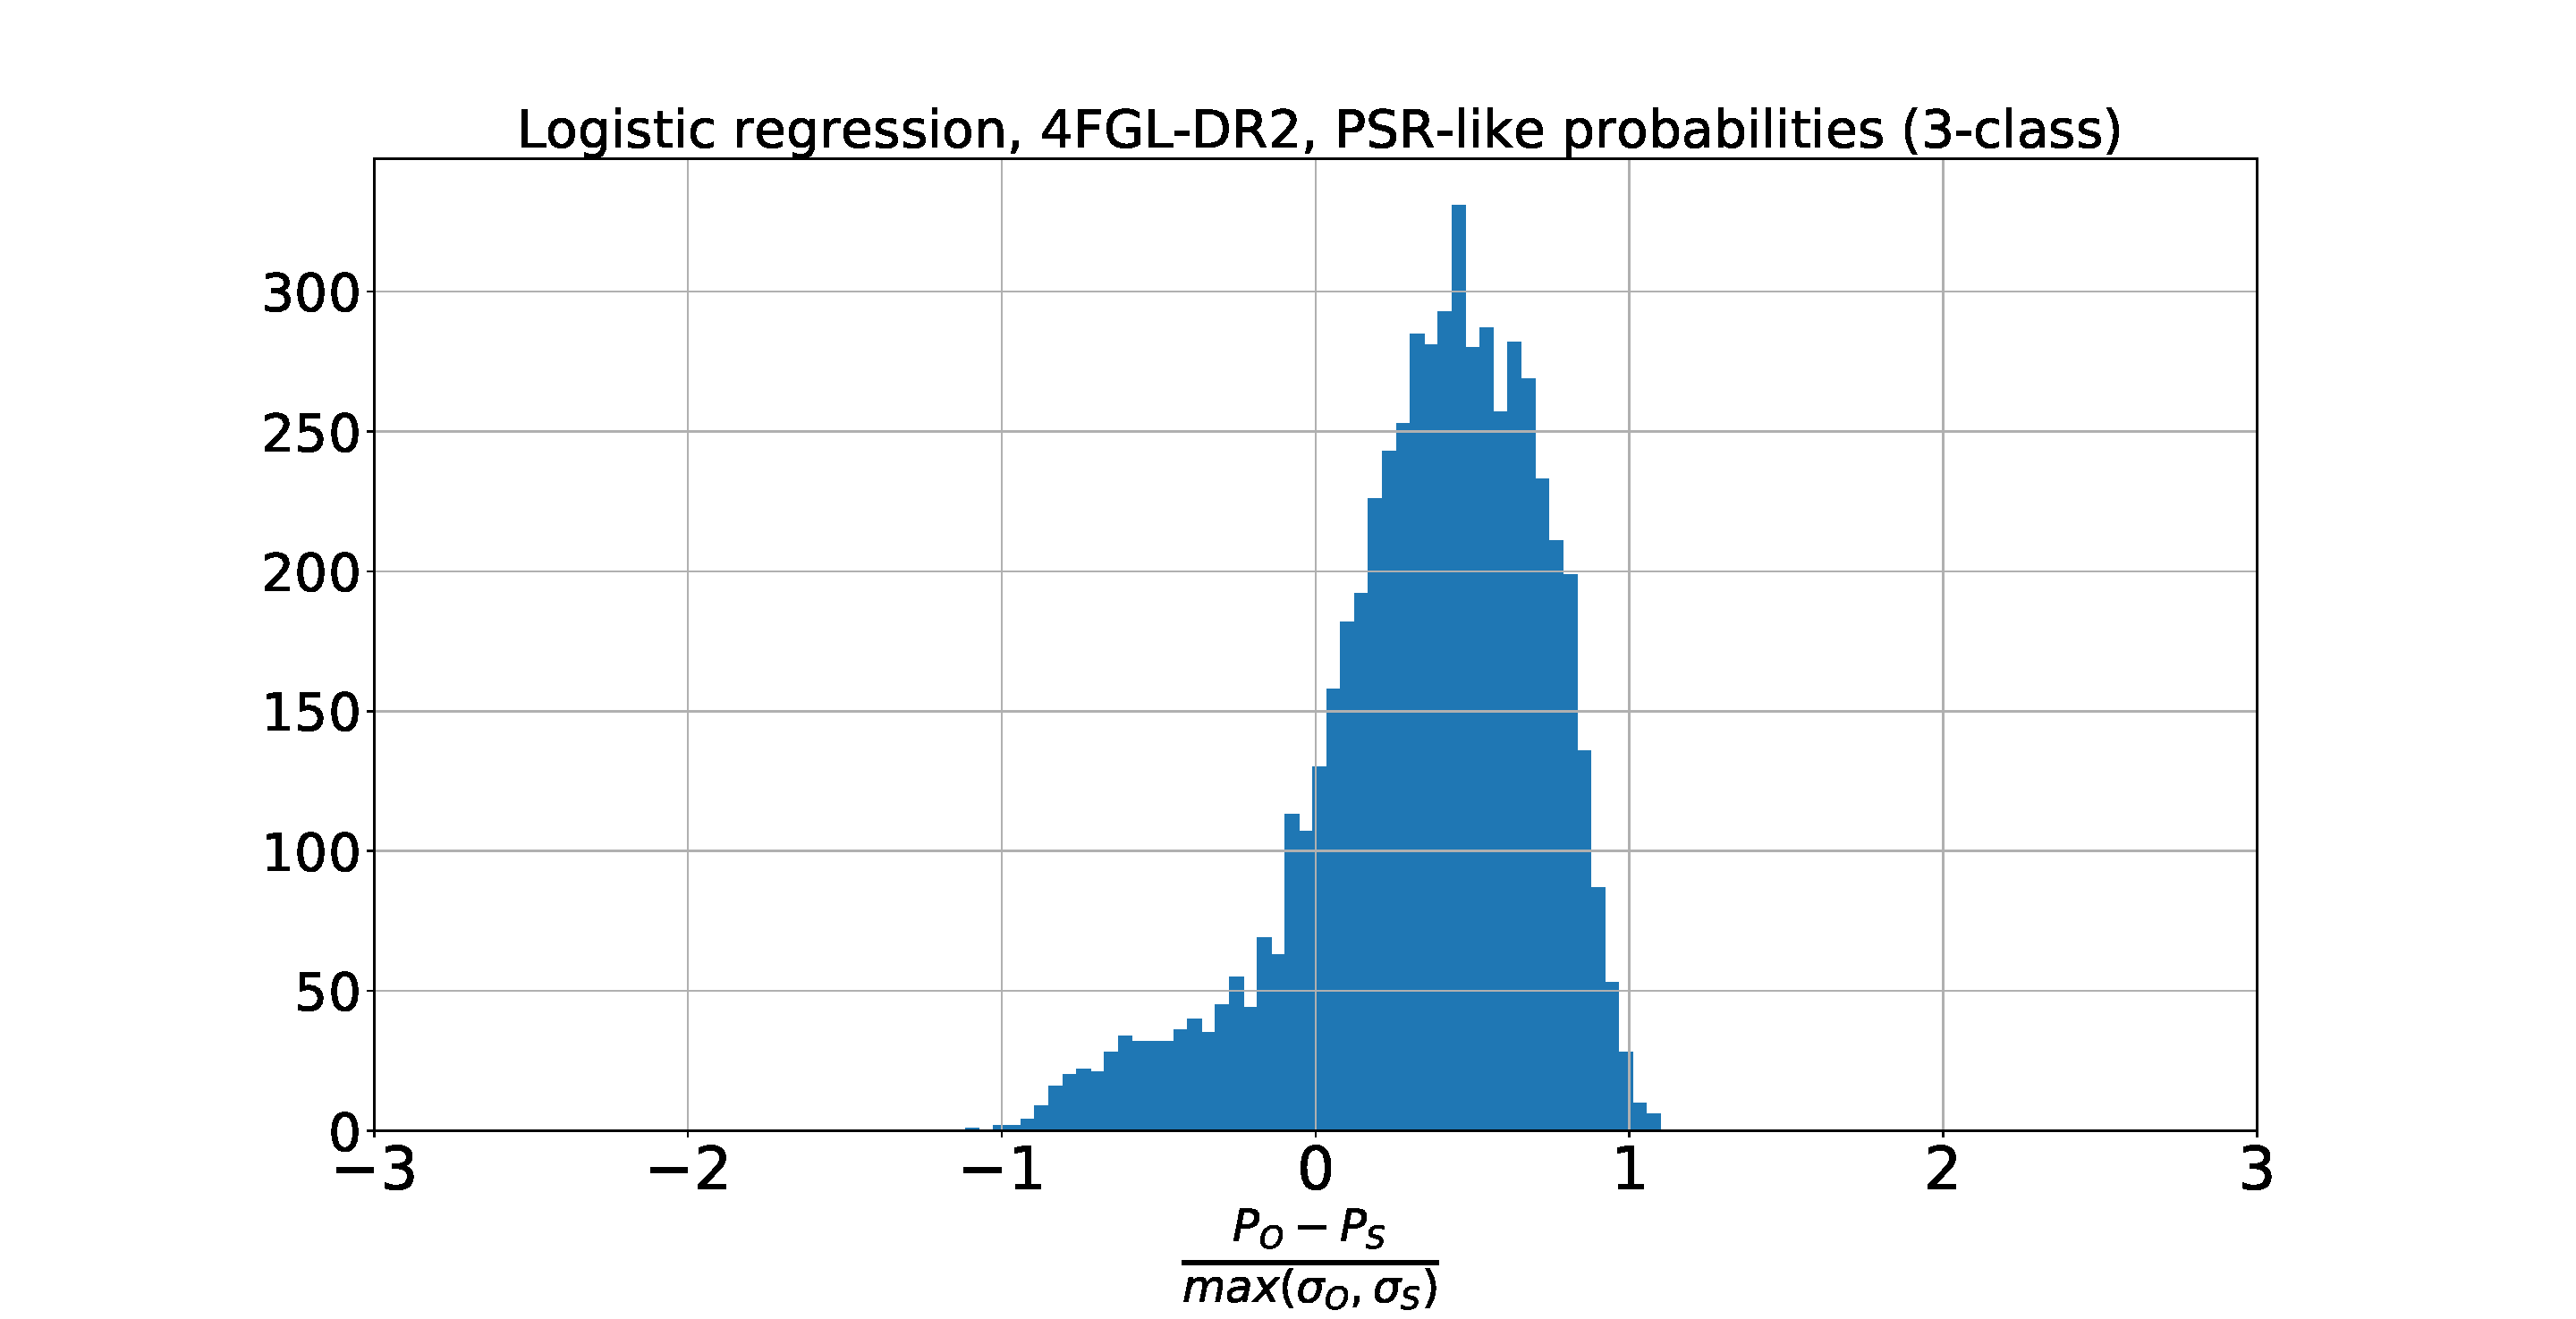
\includegraphics[width=0.55\textwidth]{plots/hist_diff_smote_LR_4FGL-DR2_3class.pdf}
\caption{Reliability diagrams for the PSR class. Top panels: 2-class classification 
taking into account only AGN and PSR associated 3FGL and 4FGL-DR2 sources.
Middle panels: same as the top panels but taking into account all associated 3FGL and 4FGL-DR2 sources.
Bottom panels: 3-class classification of 3FGL and 4FGL-DR2 sources.
}
\label{fig:rel_PSR}
\end{figure*}


\begin{figure*}[ht]
\centering
\hspace*{-0.5cm}
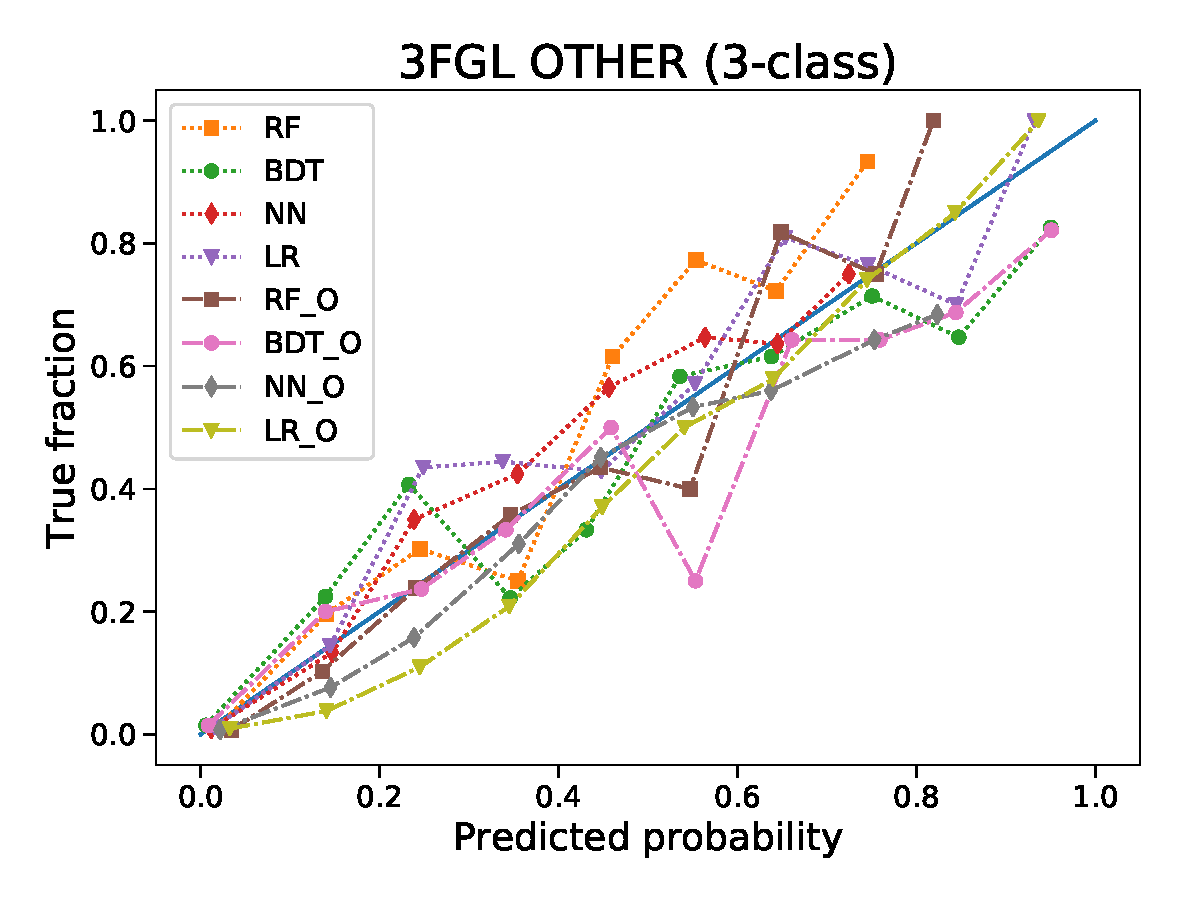
\includegraphics[width=0.45\textwidth]{plots/reliability/calibration_OTHER_3FGL_3classes.pdf}
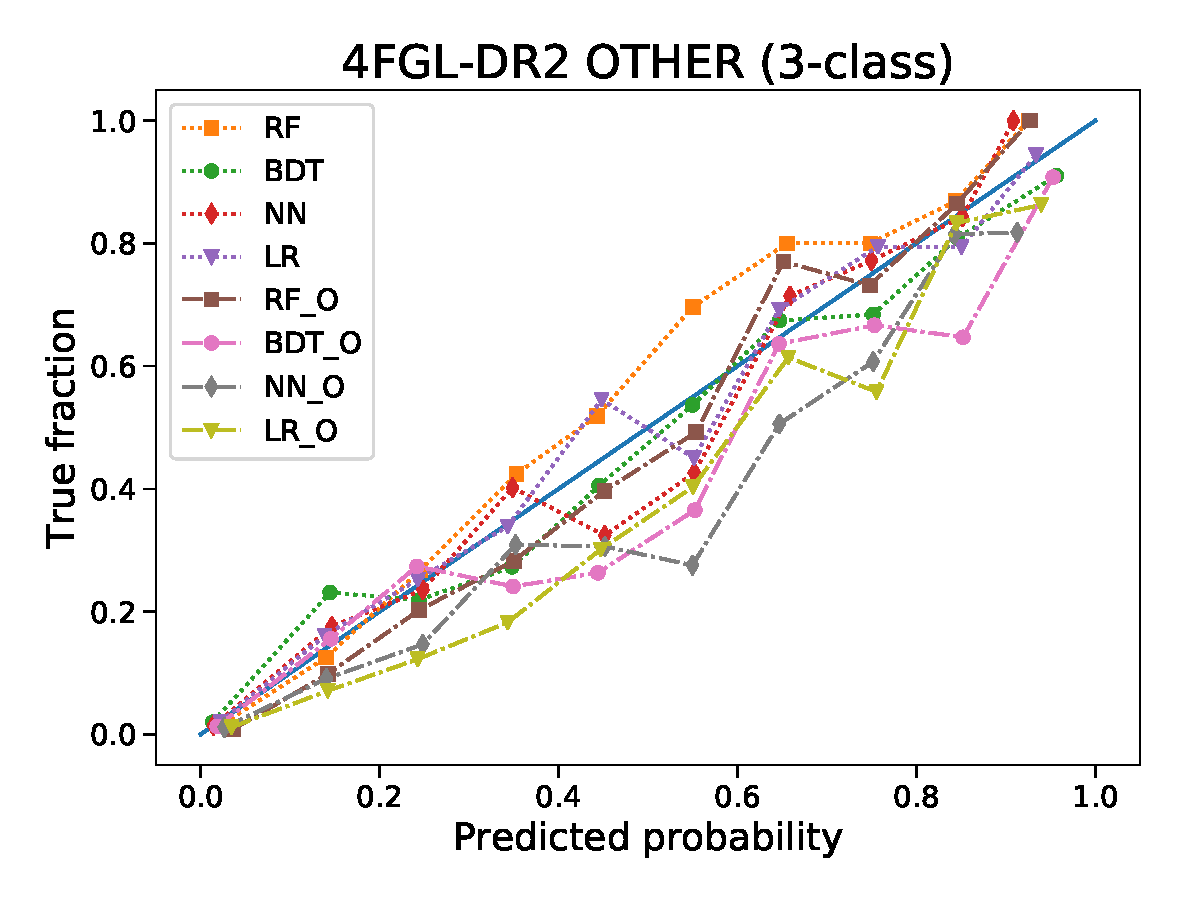
\includegraphics[width=0.45\textwidth]{plots/reliability/calibration_OTHER_4FGL-DR2_3classes.pdf}
	%\hspace*{-0.5cm}
%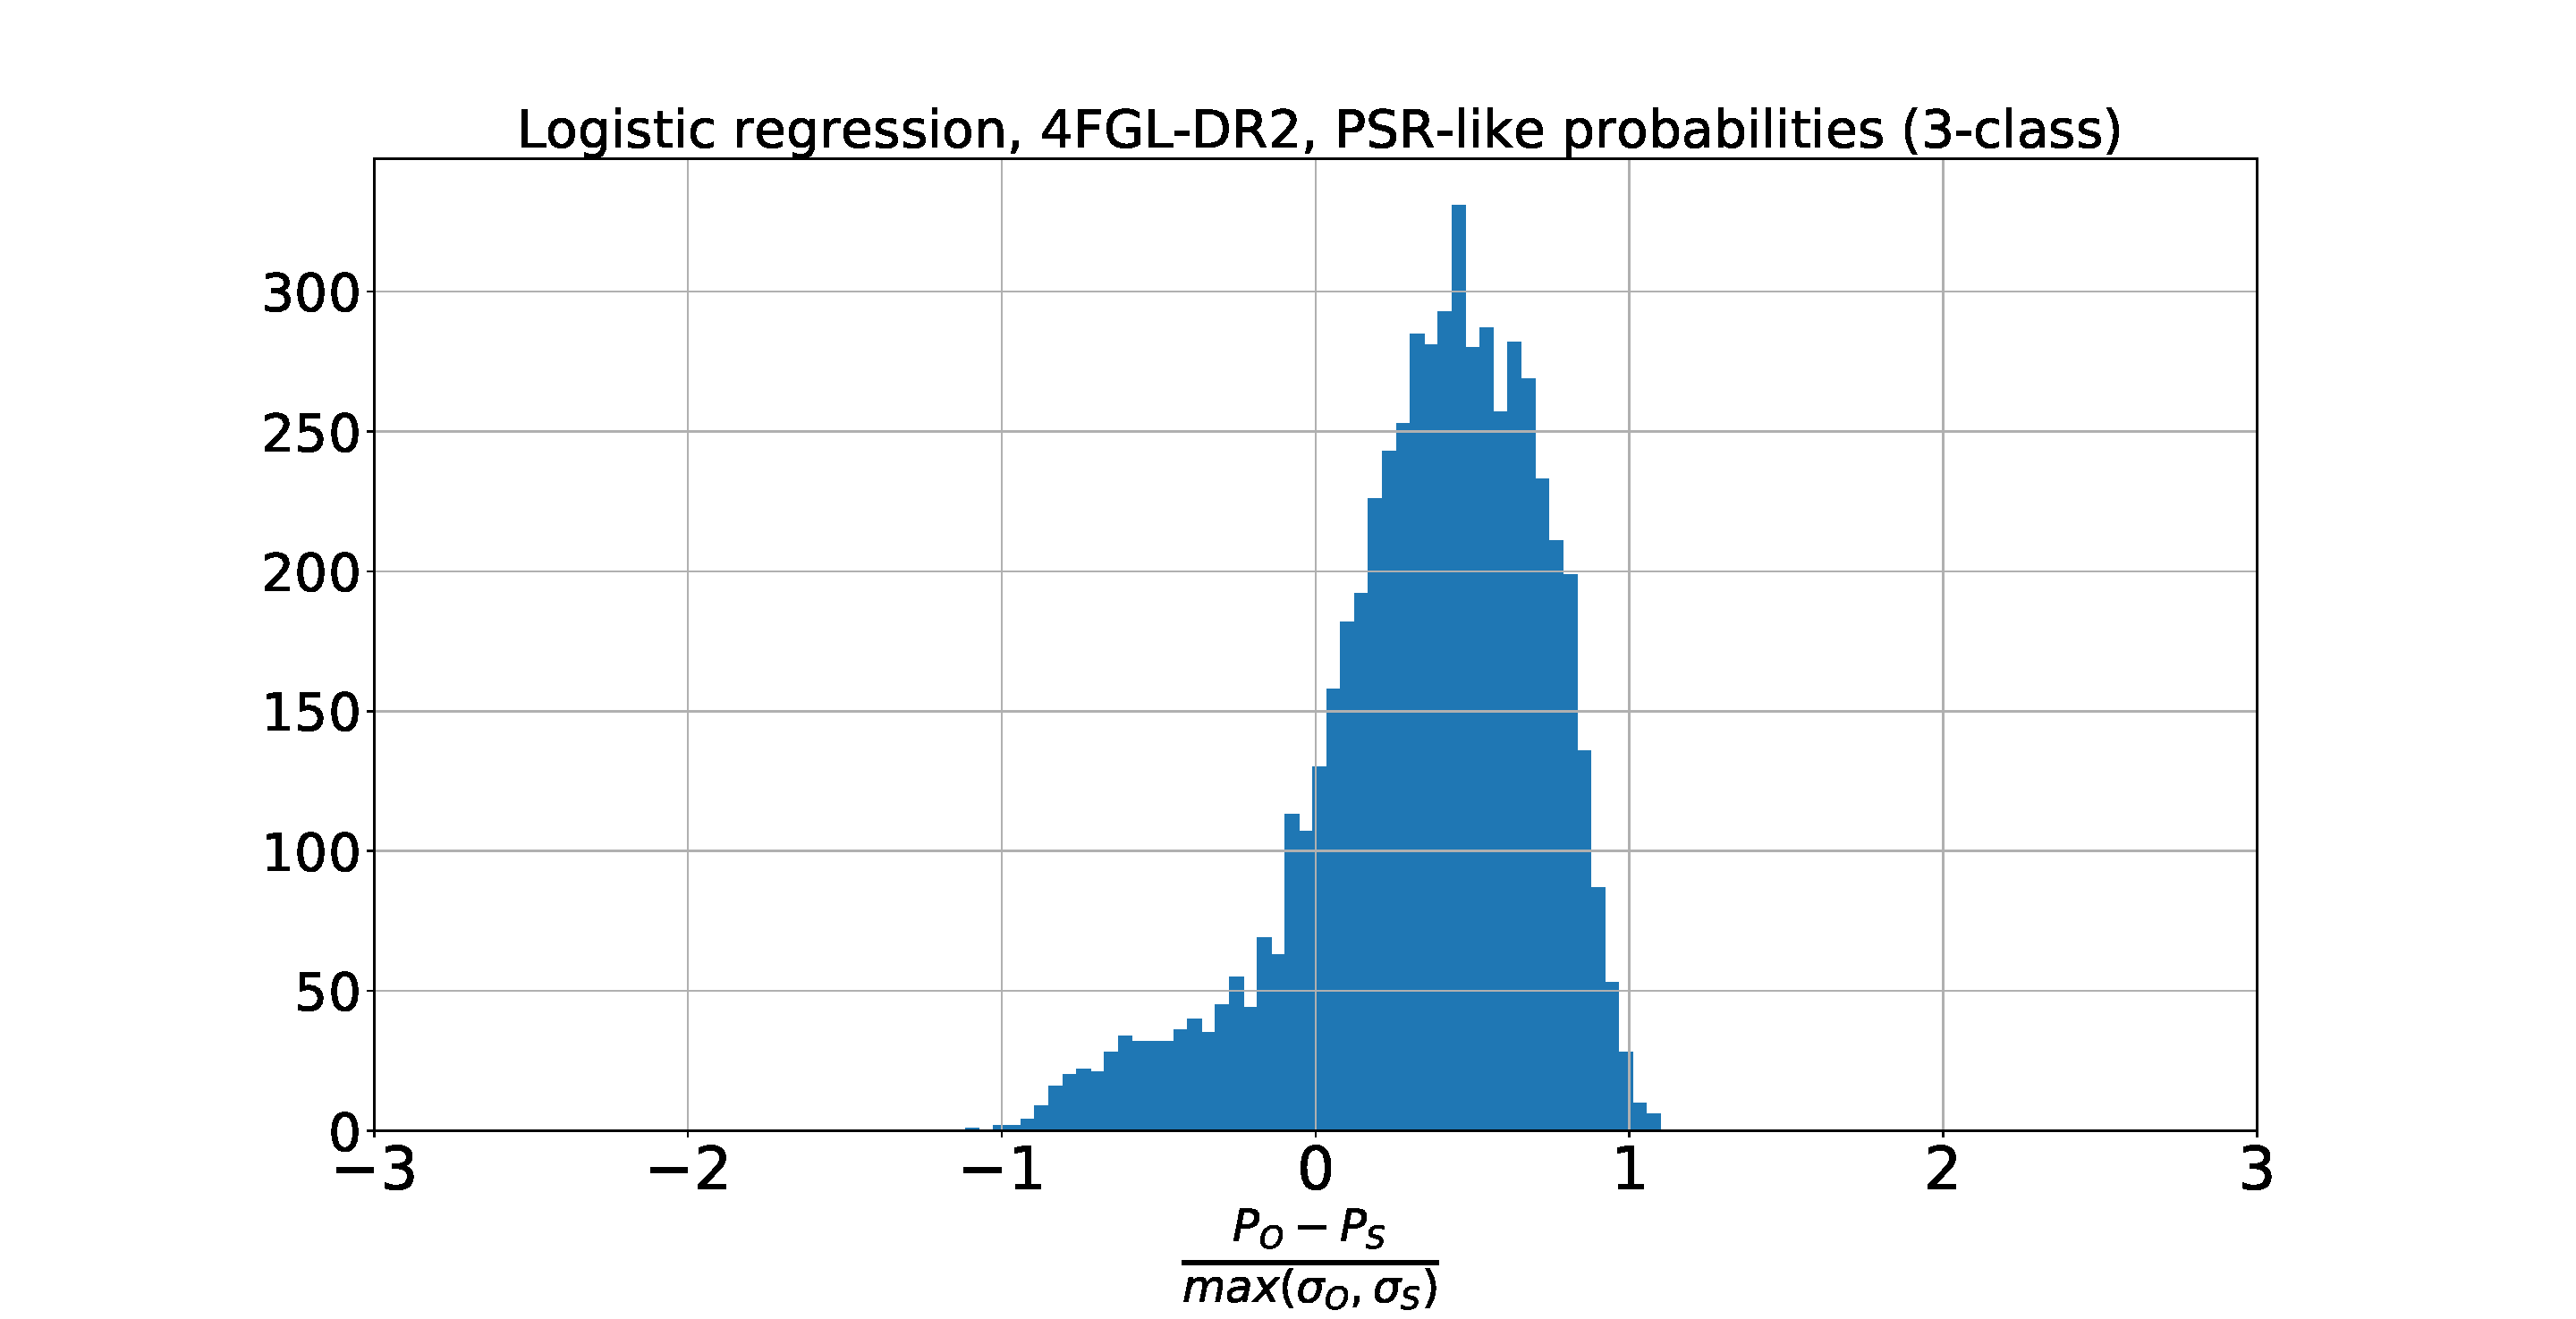
\includegraphics[width=0.55\textwidth]{plots/hist_diff_smote_LR_4FGL-DR2_3class.pdf}
\caption{Reliability diagrams for the OTHER class in the case of the 3-class classification of the 3FGL and 4FGL-DR2 sources.
}
\label{fig:rel_OTHER}
\end{figure*}

One of the characteristics of a classification algorithm is the reliability diagram (also known as the calibration curve),
where one compares predicted probabilities with the true fractions of correct classifications.
For the calculations we use ``calibration\_curve'' function implemented in scikit-learn.

In Fig. \ref{fig:rel_PSR} we show the reliability diagram for PSR classification in the 2- and 3-class cases
for the 3FGL and 4FGL-DR2 catalogs.
The predicted PSR-like probabilities for the associated sources are separated in 10 equally spaced bins between 0 and 1, 
the x-values are the average predicted probabilities in each bin,
the y-values are the fractions of associated pulsars among the sources with predicted probabilities 
in the corresponding bins.
The solid lines at $45^\circ$ show the perfect calibration, when the expected probabilities are on average equal to the 
fraction of true classifications.
If the curve is above (below) the perfect calibration line, then the expected probabilities are smaller (larger) than the true fraction,
i.e., the algorithm underestimates (overestimates) the true fraction.


In the top panels of Fig. \ref{fig:rel_PSR} we show the reliability diagrams for the 2-class classification
where we take into account only sources in PSR and AGN classes.
One can see that without oversampling, some algorithms tend to underestimate the true fraction (e.g., RF and LR in the 3FGL 2-class case),
while with oversampling, the algorithms generally overestimate the true fraction of PSRs (e.g., NN\_O and LR\_O for 3FGL and all oversampling algorithms for 4FGL-DR2) -- this behavior is not unexpected, since in the oversampling case we artificially increase the number of sources in the smaller class.

In the middle panels of Fig. \ref{fig:rel_PSR} we show the reliability diagrams  for the 2-class classification
when we add the OTHER sources.
In this case all algorithms underestimate the true fraction of PSRs, this is due to the presence of additional sources,
none of which are pulsars.
It shows that the 2-class classification is likely overestimating the number of pulsars among the unassociated sources
due to the presence of the OTHER sources.
Thus some correction or calibration is needed.

The bottom panels of Fig. \ref{fig:rel_PSR} show the reliability diagrams in the 3-class case.
One can see that the performance of the algorithms is not worse than in the 2-class case on the top panels
(the better performance of the oversampling cases can be in part attributed to fewer sources added in the oversampling
for the 3-class case).
In Fig. \ref{fig:rel_OTHER} we show the reliability diagrams for the OTHER class in the 3-class classification.
One can see that the performance of the algorithms is also good in this case, although the OTHER class is the smallest class
and has different types of sources, which can in principle lead to confusion with other classes
and poor performance of classification.

Overall, we find that the reliability of predictions in the 3-class case is similar to the performance
in the 2-class case when only PSR and AGN classes are taken into account.
In addition, we expect a similar performance for the unassociated sources, since the OTHER class is included in the 
calculation of the reliability diagrams, i.e., no correction is needed as in the 2-class case.
We also note, that although a particular algorithm can be above or below the perfect calibration curve, 
the envelope of the predictions contains the perfect calibration curve, i.e., the envelope of the predictions gives a reasonable
estimate of the modeling uncertainty.





